\documentclass[crop=false]{standalone}

\usepackage[subpreambles=false]{standalone}
\usepackage{import}
\usepackage{graphicx}
\usepackage{subcaption}
\usepackage{tikz}
\usepackage{adjustbox}
\usepackage{enumitem}

\newenvironment{rightbox}[1]
 {\itemize[
    nosep,
    leftmargin=0.1\textwidth,
    rightmargin=10pt,
    itemindent=\parindent,
    listparindent=\parindent,
  ]\item[]\relax}
 {\enditemize}

\begin{document}

\begin{figure}

  \raggedleft
  \begin{minipage}{16cm}
  \centering
  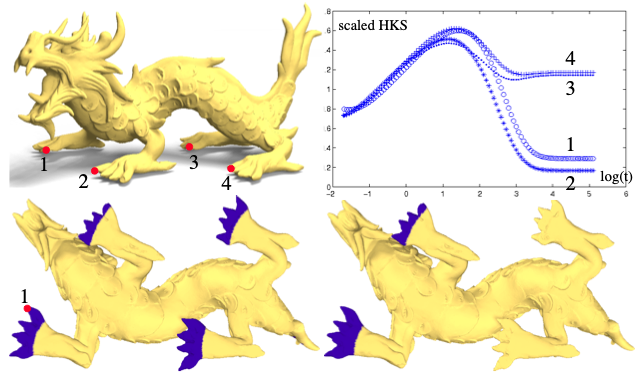
\includegraphics[width=0.65\linewidth]{thesis/appendices/import/imgs/hks_dragon.png}
  %\vspace*{-0.06\linewidth}
  \captionof{figure}{
    \textbf{Heat Kernel Signature.}
\small At four different points on a triangulated surface. For small values of t ($t < 1$), the heat kernel signature $k_t(x,x)$ is almost the same. This is, because the local geometry, i.e. the tips of the dragon's feet, is approximately equivalent. As t increases ($t > 1$), more global information is considered, and the heat kernel signatures diverge. The two points at the front and back feet still capture more common surface information about the shape than a point at the front and at the back. Image from \cite{Sun2009}.
  }
  \label{fig:hks_dragon}
  \end{minipage}
\end{figure}
\vspace{0.05\linewidth}


% \lipsum[2]
% \begin{figure}
%   \raggedleft
%   \begin{minipage}{5cm}
%   \includegraphics[width=5cm]{name}
%   \caption{Some caption that spans more than a line and some additional text}
%   \end{minipage}
% \end{figure}
\end{document}